\documentclass{beamer}
\usetheme[white]{Wisconsin}
\usepackage{longtable}
\usepackage{listings}
\usepackage{color}
%% The amssymb package provides various useful mathematical symbols
\usepackage{amssymb}
%% The amsthm package provides extended theorem environments
\usepackage{amsthm} \usepackage{amsmath} \usepackage{tmadd,tmath}
\usepackage[mathcal]{euscript} \usepackage{color}
\usepackage{textcomp}
\usepackage{algorithm,algorithmic}
\definecolor{listinggray}{gray}{0.9}
\definecolor{lbcolor}{rgb}{0.9,0.9,0.9}
\lstset{
  backgroundcolor=\color{lbcolor},
  tabsize=4,
  rulecolor=,
  language=c++,
  basicstyle=\scriptsize,
  upquote=true,
  aboveskip={1.5\baselineskip},
  columns=fixed,
  showstringspaces=false,
  extendedchars=true,
  breaklines=true,
  prebreak =
  \raisebox{0ex}[0ex][0ex]{\ensuremath{\hookleftarrow}},
  frame=single,
  showtabs=false,
  showspaces=false,
  showstringspaces=false,
  identifierstyle=\ttfamily,
  keywordstyle=\color[rgb]{0,0,1},
  commentstyle=\color[rgb]{0.133,0.545,0.133},
  stringstyle=\color[rgb]{0.627,0.126,0.941},
}

%% colors
\setbeamercolor{boxheadcolor}{fg=white,bg=UWRed}
\setbeamercolor{boxbodycolor}{fg=black,bg=white}


%%---------------------------------------------------------------------------%%
\author{Stuart R. Slattery
  \\ Engineering Physics Department
  \\ University of Wisconsin - Madison
}

\date{\today} 
\title{Domain Decomposed Monte Carlo} 
\begin{document}
\maketitle

%%---------------------------------------------------------------------------%%
\begin{frame}{Monte Carlo Linear Solver Preliminaries}

  \begin{itemize}
  \item Split the linear operator
  \end{itemize}

  \[
  \ve{H} = \ve{I} - \ve{A}
  \]

  \[
  \ve{x} = \ve{H} \ve{x} + \ve{b}
  \]

  \medskip
  \begin{itemize}
  \item Generate the \textit{Neumann series}
  \end{itemize}
  
  \[
  \ve{A}^{-1} = (\ve{I}-\ve{H})^{-1} = \sum_{k=0}^{\infty} \ve{H}^k
  \]

  \medskip
  \begin{itemize}
  \item Require $\rho(\ve{H}) < 1$ for convergence
  \end{itemize}

  \[
  \ve{A}^{-1}\ve{b} = \sum_{k=0}^{\infty} \ve{H}^k\ve{b} = \ve{x}
  \]

\end{frame}

%%---------------------------------------------------------------------------%%
\begin{frame}{Monte Carlo Linear Solver Preliminaries}

  \begin{itemize}
  \item Expand the Neumann series
  \end{itemize}

  \[
  x_i = \sum_{k=0}^{\infty}\sum_{i_1}^{N}\sum_{i_2}^{N}\ldots
  \sum_{i_k}^{N}h_{i,i_1}h_{i_1,i_2}\ldots h_{i_{k-1},i_k}b_{i_k}
  \]

  \medskip
  \begin{itemize}
  \item Define a sequence of state transitions
  \end{itemize}
  
  \[
  \nu = i \rightarrow i_1 \rightarrow \cdots \rightarrow i_{k-1}
  \rightarrow i_{k}
  \]

  \medskip
  \begin{itemize}
  \item Define the \textit{Neumann-Ulam decomposition}\footnote{The
    Hadamard product $\ve{A} = \ve{B} \circ \ve{C}$ is defined
    element-wise as $a_{ij} = b_{ij} c_{ij}$.}
  \end{itemize}

  \[
  \ve{H} = \ve{P} \circ \ve{W}
  \]

\end{frame}

%%---------------------------------------------------------------------------%%
\begin{frame}{Adjoint Method: Evolution of a Solution}

  \begin{figure}[h!]
    \begin{center}
      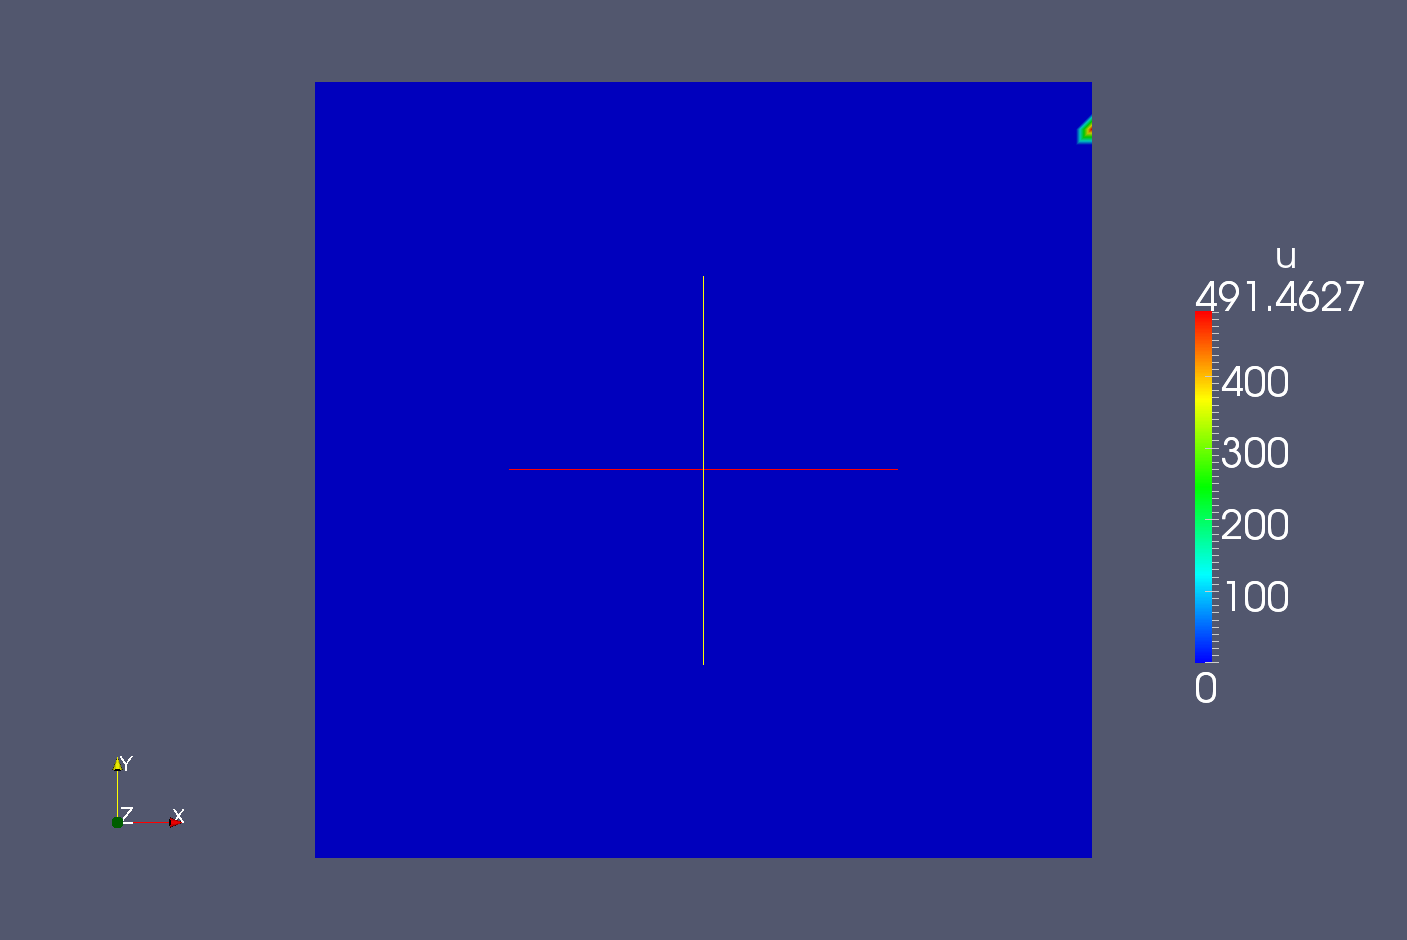
\includegraphics[width=4in]{../../prelim/presentation/adjoint_1.png}
    \end{center}
    \caption{\textbf{Adjoint solution to Poisson Equation.}
      \textit{\sn{1}{0} total histories, 0.286 seconds CPU time.} }
  \end{figure}

\end{frame}

%%---------------------------------------------------------------------------%%
\begin{frame}{Adjoint Method: Evolution of a Solution}

  \begin{figure}[h!]
    \begin{center}
      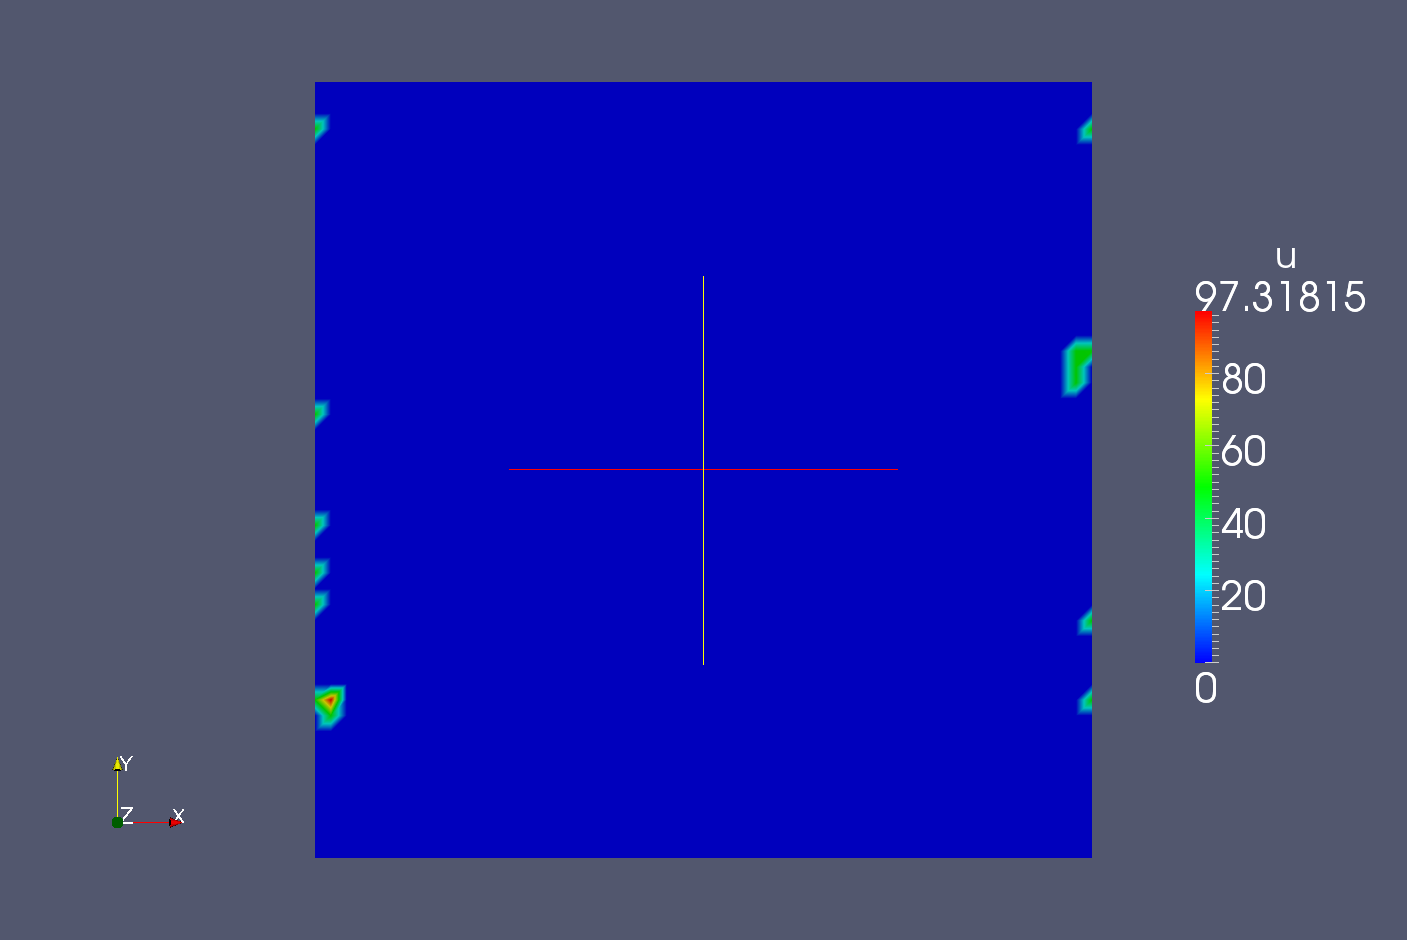
\includegraphics[width=4in]{../../prelim/presentation/adjoint_10.png}
    \end{center}
    \caption{\textbf{Adjoint solution to Poisson Equation.}
      \textit{\sn{1}{1} total histories, 0.278 seconds CPU time.} }
  \end{figure}

\end{frame}

%%---------------------------------------------------------------------------%%
\begin{frame}{Adjoint Method: Evolution of a Solution}

  \begin{figure}[h!]
    \begin{center}
      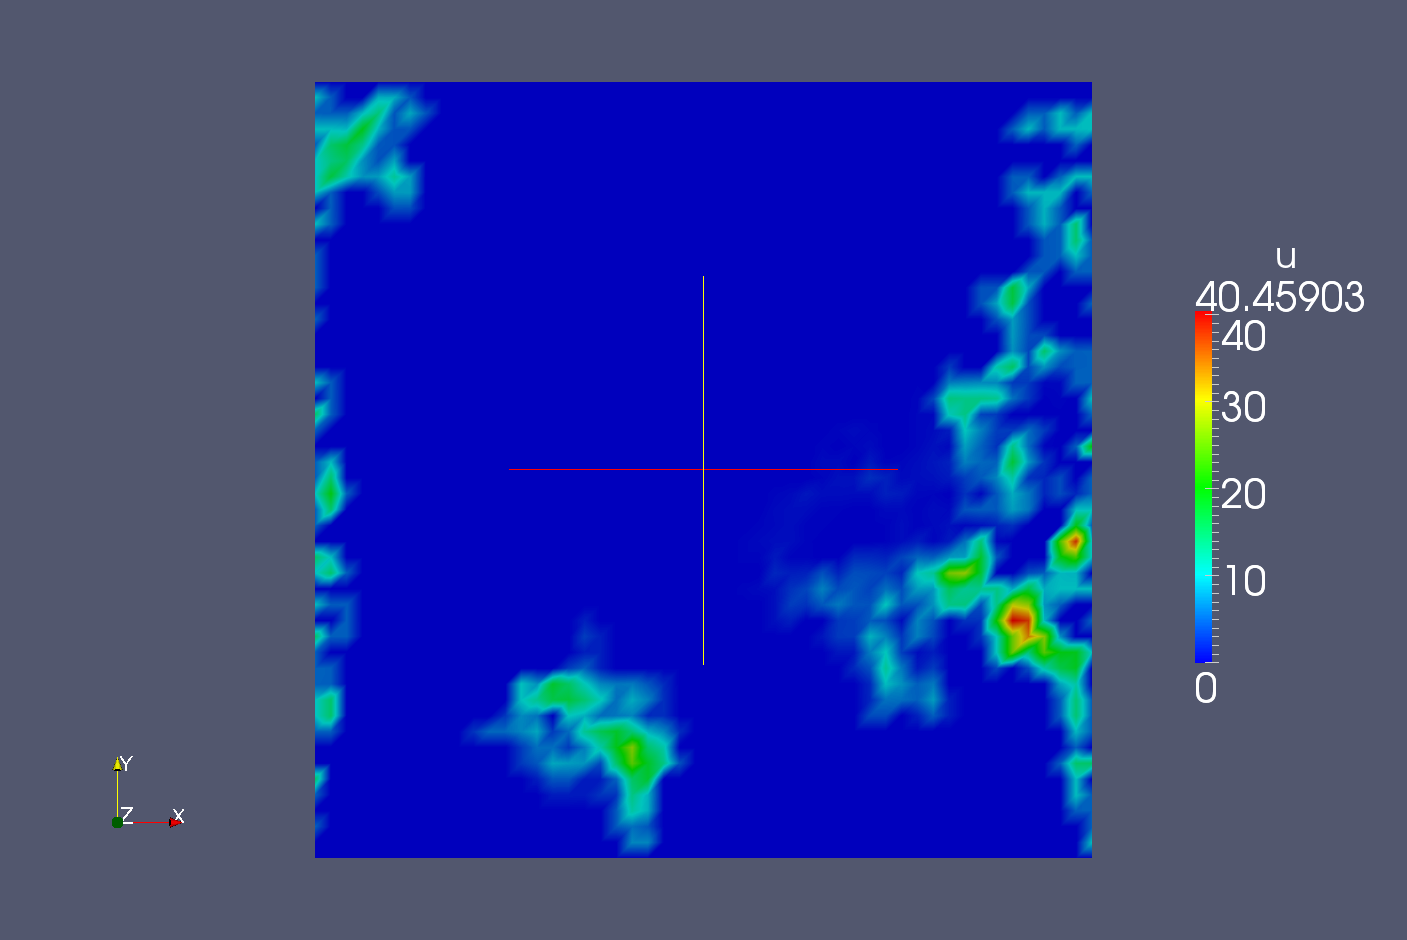
\includegraphics[width=4in]{../../prelim/presentation/adjoint_100.png}
    \end{center}
    \caption{\textbf{Adjoint solution to Poisson Equation.}
      \textit{\sn{1}{2} total histories, 0.275 seconds CPU time.} }
  \end{figure}

\end{frame}

%%---------------------------------------------------------------------------%%
\begin{frame}{Adjoint Method: Evolution of a Solution}

  \begin{figure}[h!]
    \begin{center}
      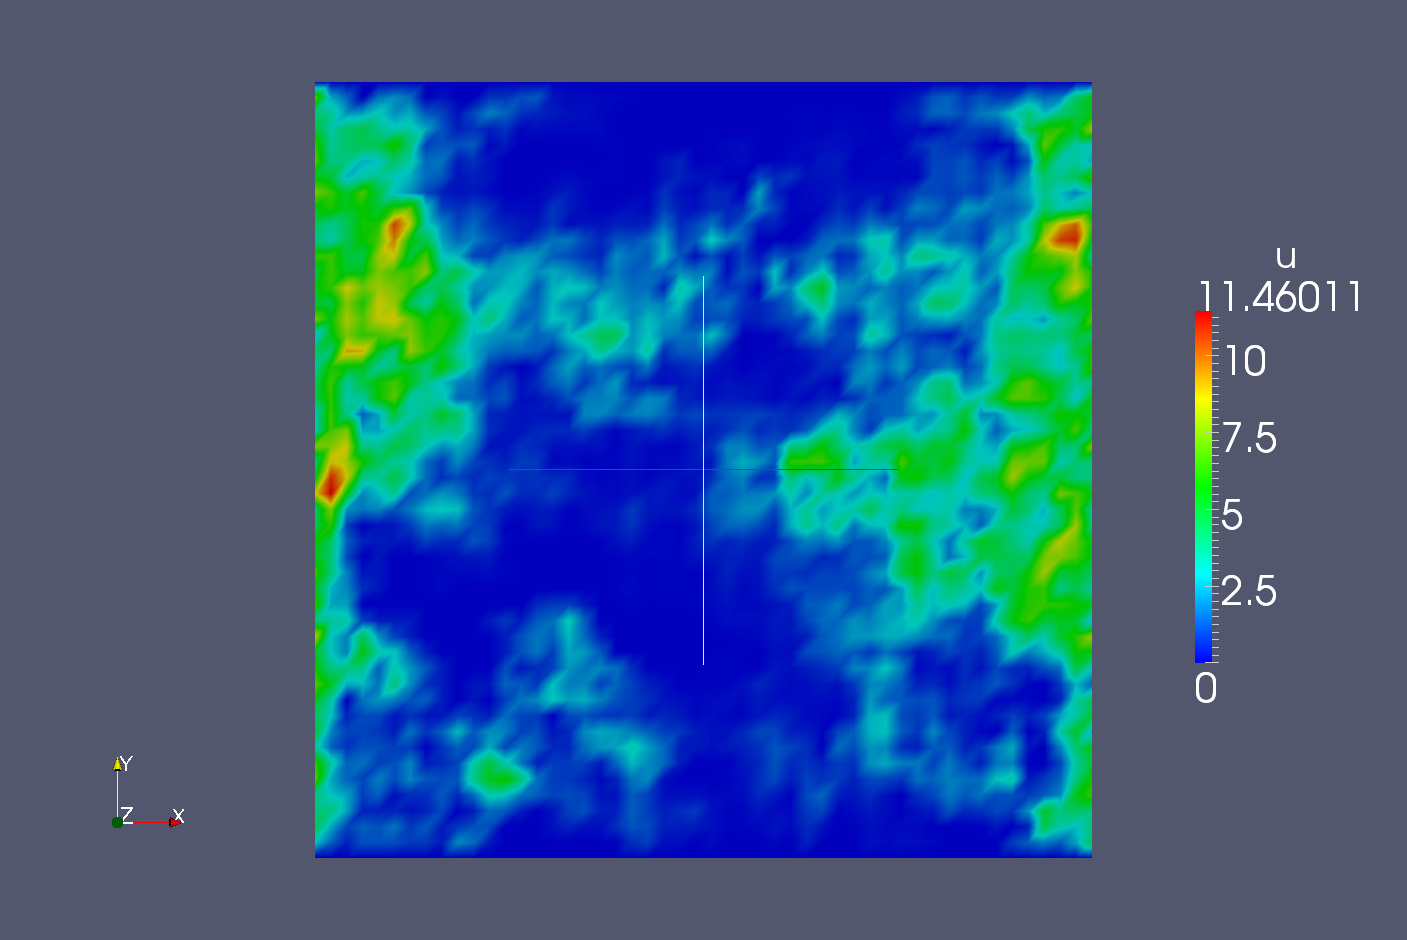
\includegraphics[width=4in]{../../prelim/presentation/adjoint_1000.png}
    \end{center}
    \caption{\textbf{Adjoint solution to Poisson Equation.}
      \textit{\sn{1}{3} total histories, 0.291 seconds CPU time.} }
  \end{figure}

\end{frame}

%%---------------------------------------------------------------------------%%
\begin{frame}{Adjoint Method: Evolution of a Solution}

  \begin{figure}[h!]
    \begin{center}
      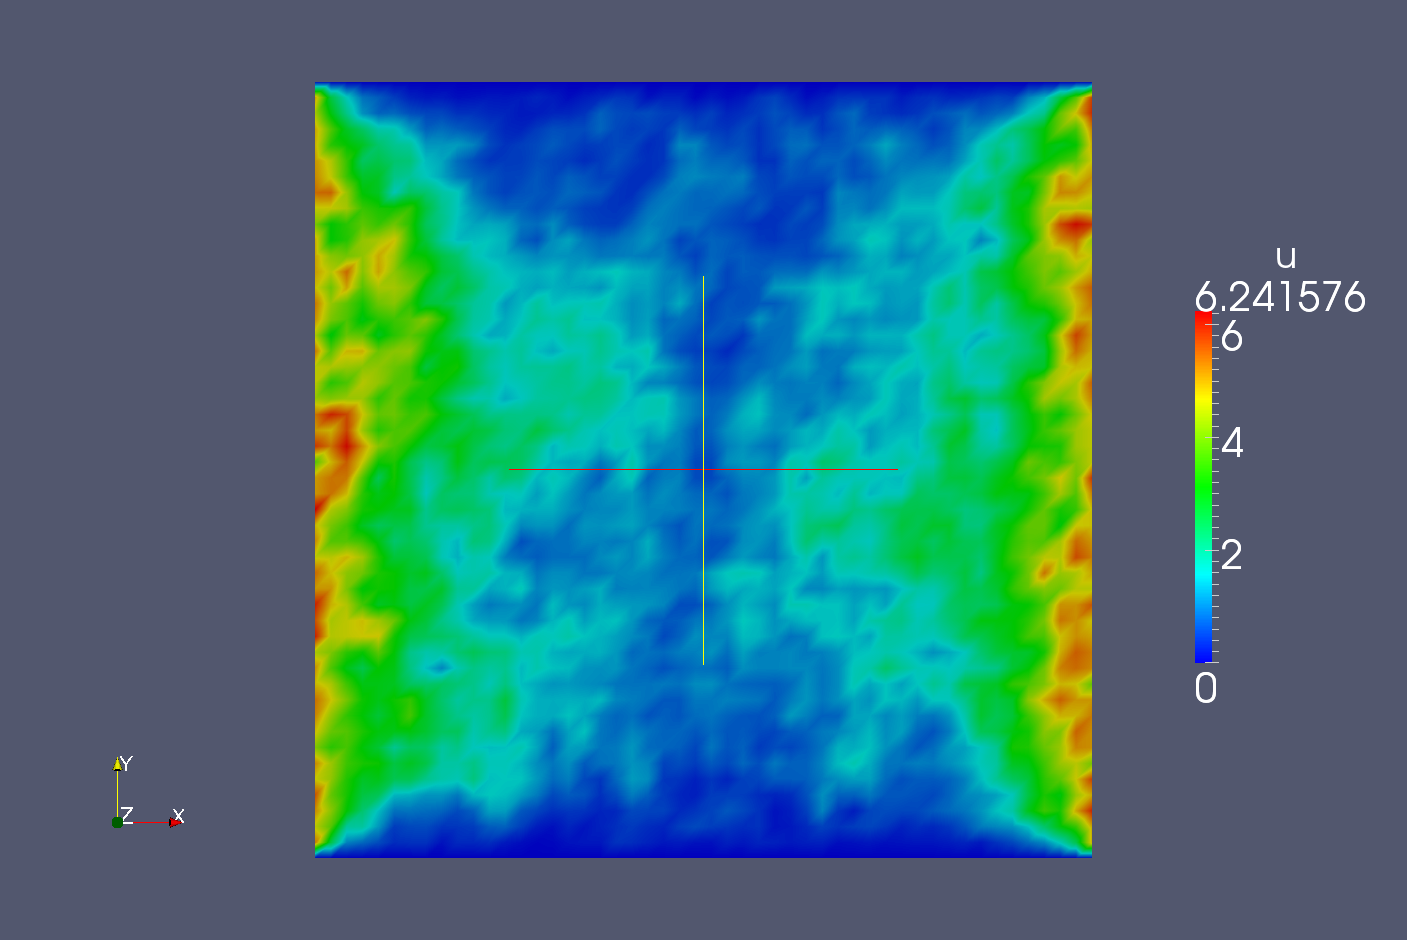
\includegraphics[width=4in]{../../prelim/presentation/adjoint_10000.png}
    \end{center}
    \caption{\textbf{Adjoint solution to Poisson Equation.}
      \textit{\sn{1}{4} total histories, 0.428 seconds CPU time.} }
  \end{figure}

\end{frame}

%%---------------------------------------------------------------------------%%
\begin{frame}{Adjoint Method: Evolution of a Solution}

  \begin{figure}[h!]
    \begin{center}
      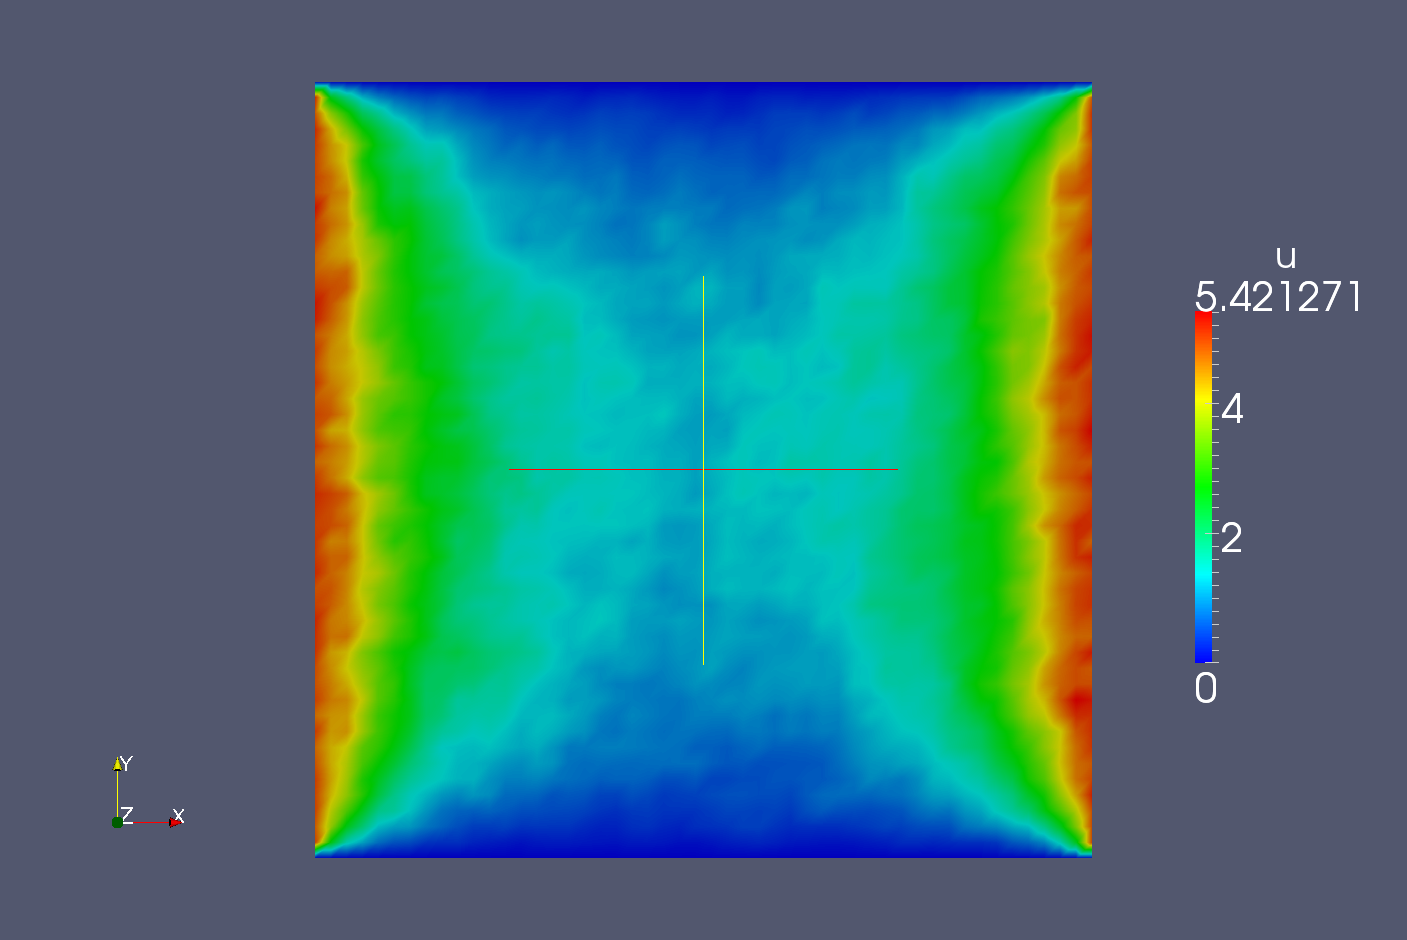
\includegraphics[width=4in]{../../prelim/presentation/adjoint_100000.png}
    \end{center}
    \caption{\textbf{Adjoint solution to Poisson Equation.}
      \textit{\sn{1}{5} total histories, 1.76 seconds CPU time.} }
  \end{figure}

\end{frame}

%%---------------------------------------------------------------------------%%
\begin{frame}{Adjoint Method: Evolution of a Solution}

  \begin{figure}[h!]
    \begin{center}
      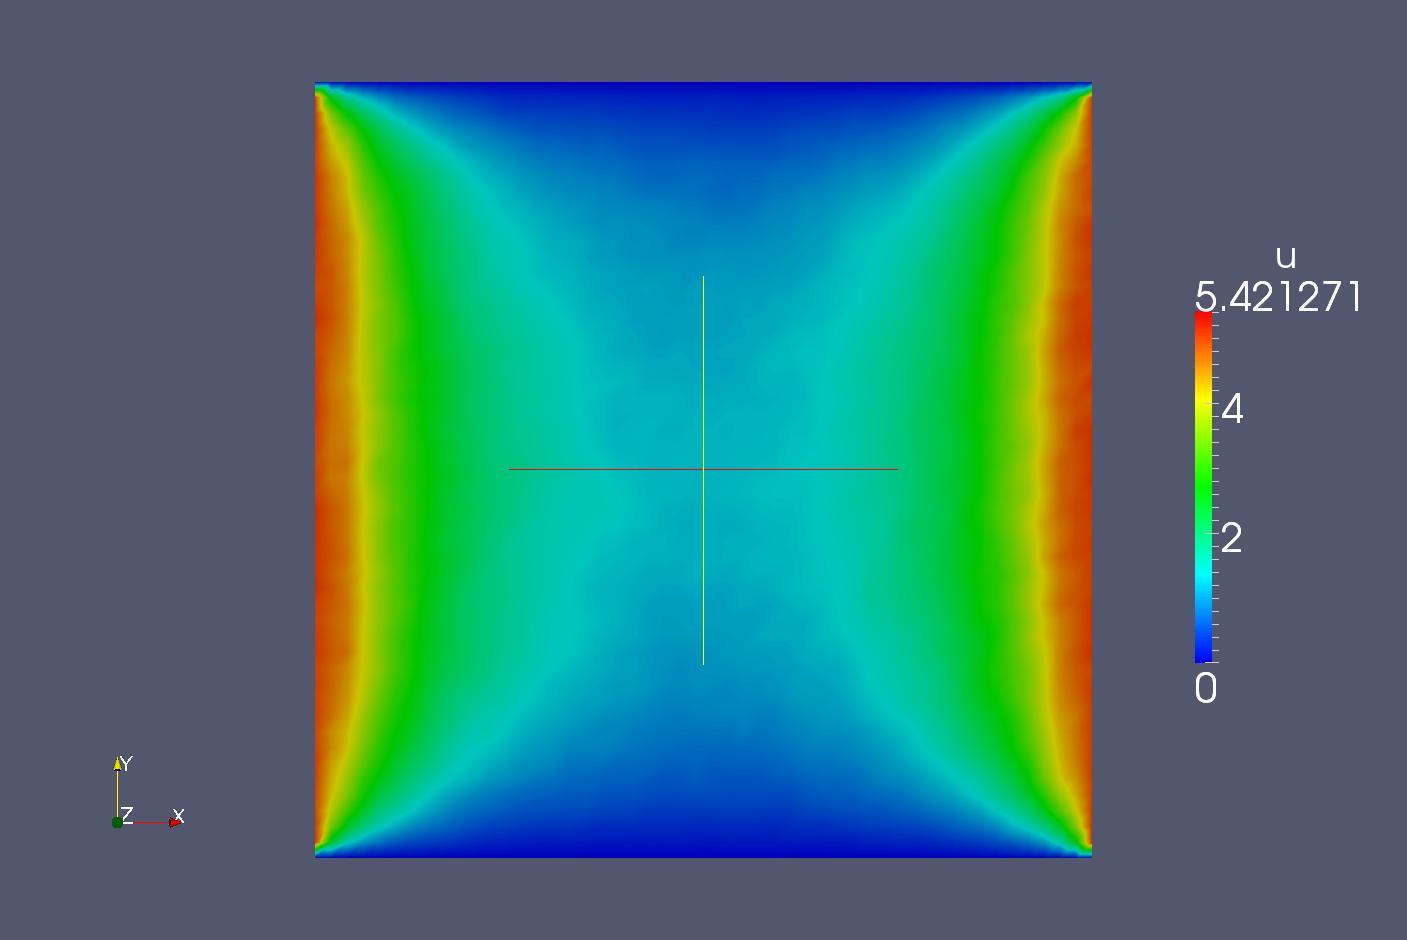
\includegraphics[width=4in]{../../prelim/presentation/adjoint_1000000.png}
    \end{center}
    \caption{\textbf{Adjoint solution to Poisson Equation.}
      \textit{\sn{1}{6} total histories, 15.1 seconds CPU time.} }
  \end{figure}

\end{frame}

%%---------------------------------------------------------------------------%%
\begin{frame}{Adjoint Method: Evolution of a Solution}

  \begin{figure}[h!]
    \begin{center}
      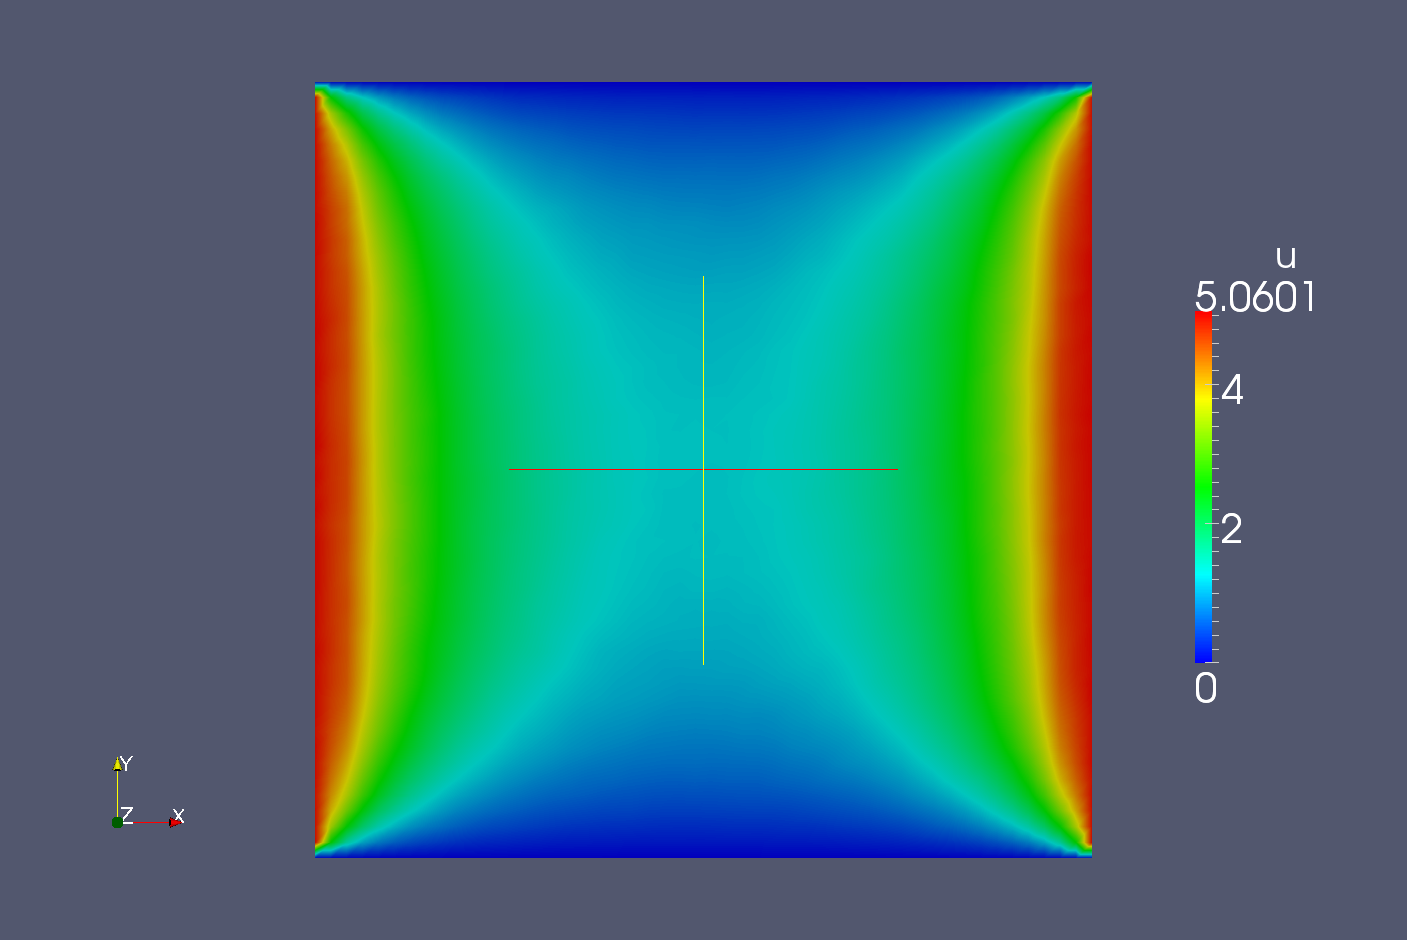
\includegraphics[width=4in]{../../prelim/presentation/adjoint_10000000.png}
    \end{center}
    \caption{\textbf{Adjoint solution to Poisson Equation.}
      \textit{\sn{1}{7} total histories, 149 seconds CPU time.} }
  \end{figure}

\end{frame}

%%---------------------------------------------------------------------------%%
\begin{frame}{Parallelization of Monte Carlo Methods}

  \begin{itemize}
  \item No literature observed for parallel Neumann-Ulam solvers
    \medskip \medskip
  \item Numerous references for modern parallel Monte Carlo methods in
    reactor physics
    \medskip \medskip
  \item Build a strategy for applying modern methods to the
    Neumann-Ulam method
  \end{itemize}

\end{frame}

%%---------------------------------------------------------------------------%%
\begin{frame}{Domain Decomposition}

  \begin{itemize}
  \item Each parallel process owns a piece of the domain
  \item Random walks must be transported across domains through
    communication
  \end{itemize}

  \medskip \medskip
  \begin{beamerboxesrounded}[upper=boxheadcolor,lower=boxbodycolor,shadow=true]
    {Brunner's Work (2006 and 2009)}

    \begin{itemize}
    \item Looked at 4 communication patterns:
      \begin{itemize}
      \item Fully-locking synchronous
      \item Asynchronous-send/synchronous-receive
      \item Master/slave
      \item Binary tree master/slave
      \end{itemize}
    \item Binary tree master/slave performed best but race conditions observed
    \item A later improvement to their work showed a fully asynchronous
      pattern to work best
    \item Poor scaling for unbalanced problems for all schemes
    \end{itemize}
    
  \end{beamerboxesrounded}

\end{frame}

%%---------------------------------------------------------------------------%%
\begin{frame}{Domain Decomposition}
\end{frame}

%%---------------------------------------------------------------------------%%
\begin{frame}{Fully Synchronous Algorithm}
\end{frame}

%%---------------------------------------------------------------------------%%
\begin{frame}{Fully Asynchronous Algorithm}
\end{frame}

%%---------------------------------------------------------------------------%%
\begin{frame}{Brunner's Communication Parameters}

  \begin{figure}[h!]
    \begin{center}
      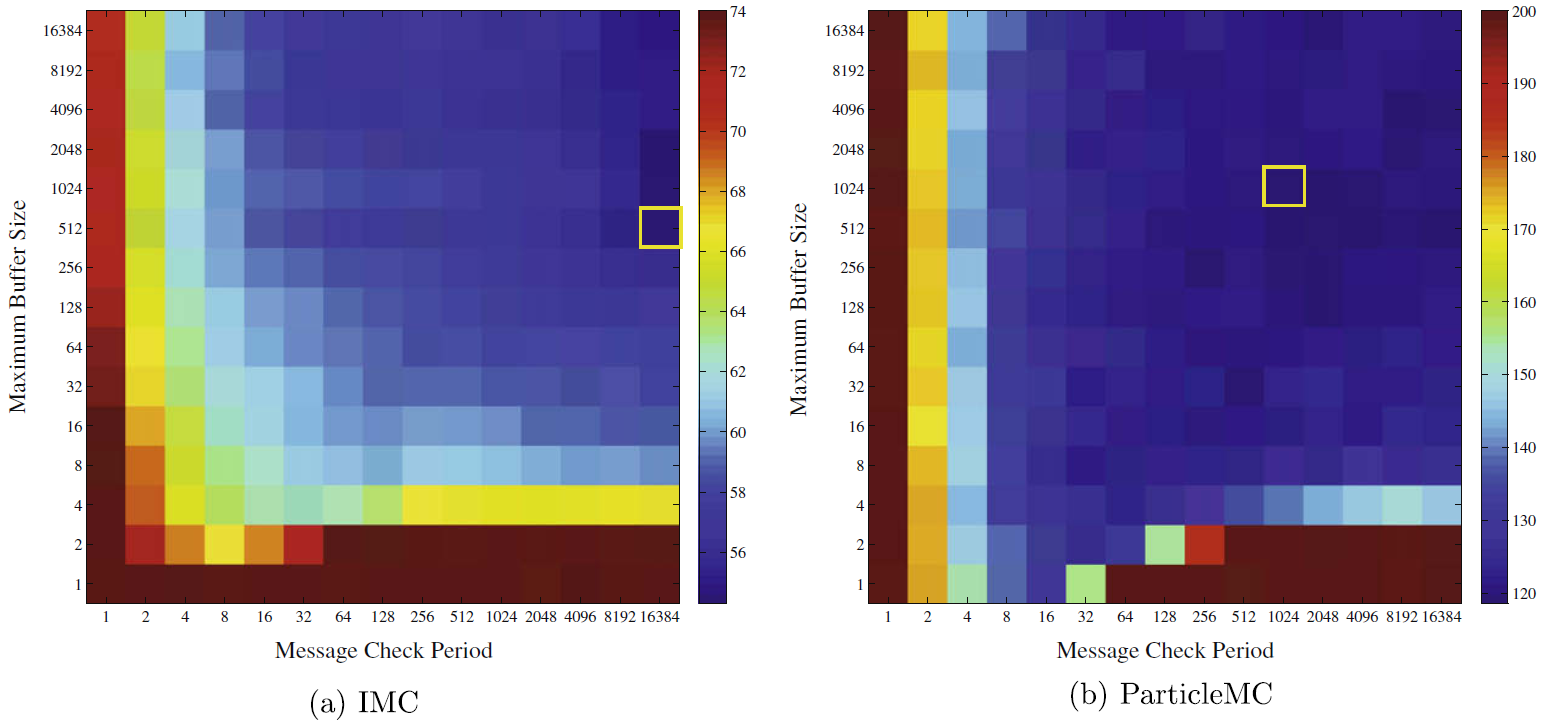
\includegraphics[width=5in]{brunner_params.png}
    \end{center}
  \end{figure}

\end{frame}

%%---------------------------------------------------------------------------%%
\begin{frame}{My Communication Parameters}

  \begin{figure}[h!]
    \begin{center}
      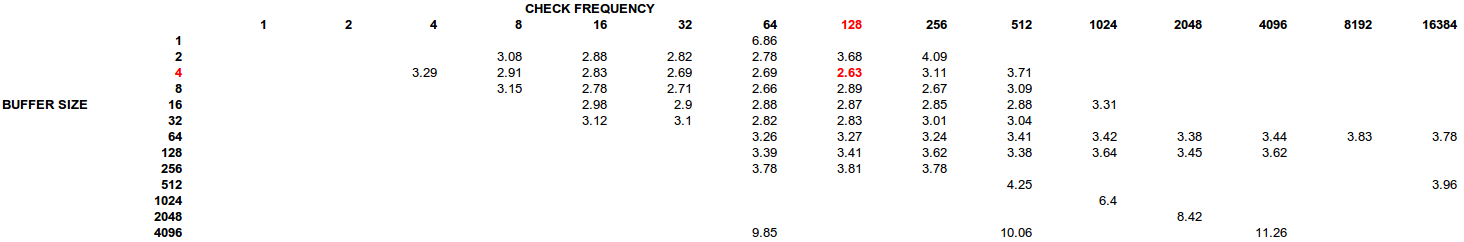
\includegraphics[width=5in]{my_params.png}
    \end{center}
  \end{figure}

\end{frame}

%%---------------------------------------------------------------------------%%
\begin{frame}{Brunner's Strong Scaling}

  \begin{figure}[h!]
    \begin{center}
      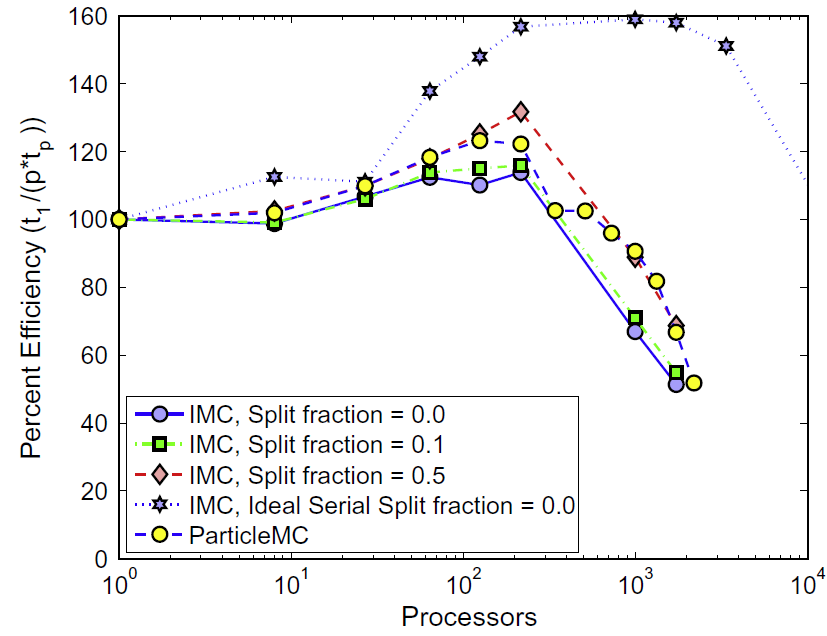
\includegraphics[width=4in]{brunner_strong.png}
    \end{center}
  \end{figure}

\end{frame}

%%---------------------------------------------------------------------------%%
\begin{frame}{My Strong Scaling}

  \begin{figure}[h!]
    \begin{center}
      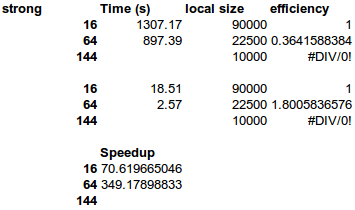
\includegraphics[width=4in]{my_strong.png}
    \end{center}
  \end{figure}

\end{frame}

%%---------------------------------------------------------------------------%%
\begin{frame}{Brunner's Weak Scaling}

  \begin{figure}[h!]
    \begin{center}
      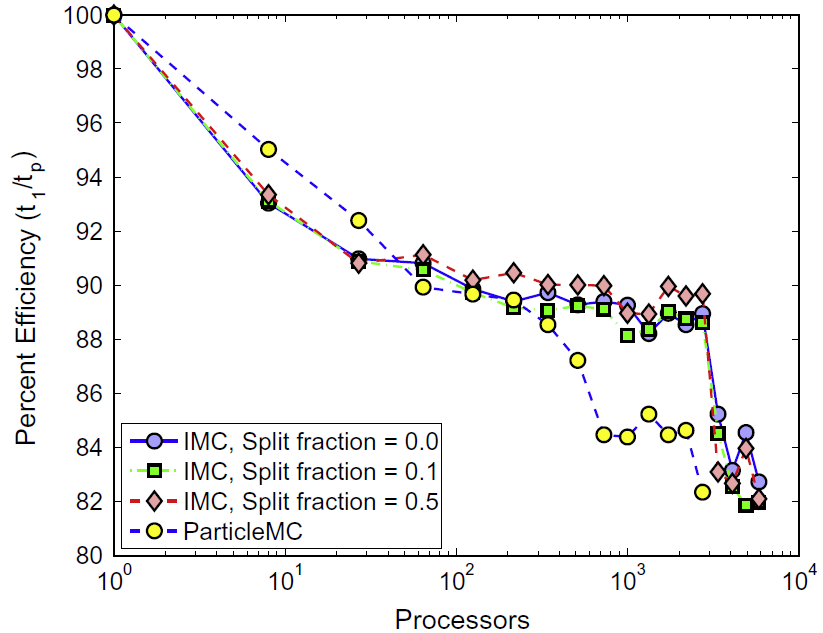
\includegraphics[width=4in]{brunner_weak.png}
    \end{center}
  \end{figure}

\end{frame}

%%---------------------------------------------------------------------------%%
\begin{frame}{My Weak Scaling}

  \begin{figure}[h!]
    \begin{center}
      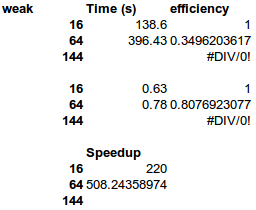
\includegraphics[width=4in]{my_weak.png}
    \end{center}
  \end{figure}

\end{frame}

%%---------------------------------------------------------------------------%%

\end{document}
